\chapter{Kontext vyhodnocování výkonu}

\section{Automatické vyhodnocování}
Ve scénáři z minulé kapitoly byl zmíněn problém programátora s~testováním výkonu. Programátor má unit
testy, které testují korektnost jeho softwaru. Umí je efektivně spouštět s~každou změnou
pomocí průběžné integrace. Chtěl by, aby mohl podobně efektivně testovat i~výkon svého softwaru.

S~testováním výkonu je ale problém. Když se spustí měření výkonu, tak výsledkem je pouhá
datová sada. Tato datová sada nevypovídá nic o~změně průběžného výkonu, která
je zajímavá. Právě podle změny ve~výkonu softwaru je možné zjistit, jestli je nutné
kód optimalizovat, protože dochází k~významným zhoršením.

Při měření výkonu dochází jako při jakémkoli jiném měření k šumu. Tento šum se projevuje
tak, že pokud se měření opakuje při~stejných podmínkách, tak se naměřené hodnoty liší.
Tomuto šumu se nelze vyvarovat. Měření proto opakujeme a naměřené hodnoty vyhodnocujeme
pomocí statistických metod, které si s~tímto šumem poradí.

Vyvinutý systém PerfEval řeší programátorův problém. Jedná se o~nástroj, který může
zakomponovat do~své průběžné integrace tak, aby byl pokles výkonu hlášen. Nástroj
při~spuštění průběžné integrace porovná dvě poslední verze a~případně oznámí zhoršení výkonu.
Na~základě tohoto hlášení může celá průběžná integrace hlásit varování nebo zprávu o~chybě, což je obdobné chování,
jako se očekává při selhání unit testů.

\section{Měření výkonu}

Před začátkem vývoje PerfEvalu bylo nutné zamyslet nad tím, jak můžou výsledky měření výkonu softwaru vypadat.
V následujících odstavcích budou zmiňovány jednotlivé poznatky o výsledcích měření výkonu.
Tyto poznatky vedly k tomu, jak se PerfEval chová a jakou má architekturu.

\bigskip
\noindent\textbf{Měřené veličiny.} Testovací frameworky umožňují měřit mnoho různých fyzikálních veličin. Patří mezi ně například
doba vykonávání metody, frekvence počtu operací za jednotku času a spotřeba paměti.
Předpokládat se tedy dá jen to, že pokud vezmu dva výsledky měření výkonu ze~dvou různých
verzí, tak budou reprezentovány stejnou fyzikální veličinou a~v~lepším případě budou mít
i~stejnou fyzikální jednotku. Je tedy vhodné, aby výsledný systém byl schopen přijmout
jakoukoli veličinu bez ohledu na jednotku.

\bigskip
\noindent\textbf{Identifikátory testů.} Protože testovací frameworky nepoužívají žádné identifikátory testů, tak je nejpřímější
řešení k~jejich rozpoznávání používat jména testovacích metod jako identifikátor. Tato jména poskytují ve~výsledcích
měření jak framework BenchmarkDotNet, tak framework JMH. Z~dokumentace frameworku Criterion \cite[]{criterion}
pro měření výkonu v~jazyce~Rust se název metody ve~výsledcích nachází také. Z~toho lze
usoudit, že použití jména metody jako identifikátoru může být dostatečně obecné.

\bigskip
\noindent\textbf{Kompilace just-in-time.} V~případě měření výkonu u jazyků, které jsou kompilované metodu JIT, je nutné být obezřetný. Je nutné
všímat si, jaká data byla naměřena. Jazyky kompilované metodou JIT mohou při měření podléhat tzv. zahřívací
fázi. Jedná se o~fázi, kdy kód ještě není plně optimalizovaný, ale již se provádí a~může být měřen.
V~závislosti na použitém měřícím frameworku je pak nutné naměřená data vhodně filtrovat. V~případě, že
by se data před a~po~optimalizaci nacházela v~jedné sadě dat, mohla by být zkreslená.

\subsection{Výstup měření BenchmarkDotNet}

BenchmarkDotNet je framework určený k~měření výkonu programů na~platformě .NET. V~důsledku
toho, že měří programy na platformě .NET, je schopen měřit výkon programů napsaných
v~programovacích jazycích C\#, F\# a~Visual Basic. Podrobnosti o~tomto měřícím frameworku
je možné nalézt v~dokumentaci \cite[]{benchmarkDotNet}.

Při~měření výkonu pomocí BenchmarkDotNet se měřené hodnoty vypisují na~standardní výstup
včetně konečného shrnutí. Mimo standardní výstup se ještě výsledky měření ukládají
do~strojově zpracovatelných formátů, jako je například JSON nebo CSV.

Výstupem měření výkonu programu v~jazyce C\# pomocí frameworku BenchmarkDotNet jsou již statisticky zpracované hodnoty.
Aby bylo možné sledovat jednotlivé naměřené hodnoty, je nutné zvolit již při~psaní testů správný
exportér, který tuto funkci podporuje. Dále je nutné naměřené hodnoty filtrovat, protože C\# je kompilovaný
metodou JIT.

\begin{figure}[!ht]
    \centering
    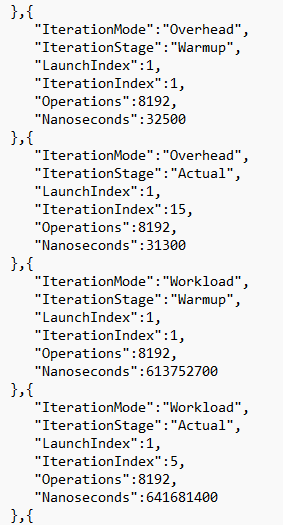
\includegraphics[width=0.3\textwidth]{../img/BenchmarkDotNET-modes.png}
    \caption{Struktura výsledků měření frameworku BenchmarkDotNET}
\end{figure}

BenchmarkDotNet je možné nakonfigurovat tak, aby se v~souboru s~výsledky nacházely podrobnosti o~prostředí, jako je operační systém,
verze platformy .NET, jméno, typ a~parametry procesoru. Dále aby se v~souboru s~výsledky nacházely
výsledky jednotlivých provedených měření. Výsledek měření u~sebe má informaci o~jméně
testovací metody, zpracované statistické údaje a~naměřené hodnoty z~různých módů a~iterací měření.
Konkrétní příklad toho, jak vypadají módy a~iterace měření se nachází na obrázku 2.1.
Názvy módů a~iterací mají intuitivní názvy, takže je z~nich poznat, kdy se ještě probíhá
překlad, a~kdy už se měří plně přeložený kód.

\subsection{Výstup měření JMH}

JMH je framework pro měření výkonu, který umožňuje pomocí anotací definovat výkonnostní testy
pro programy v~jazyce Java. Z~průzkumu \cite[]{unitTestingPerformanceSurvey} vyplývá, že se jedná o~nejpoužívanější framework
pro měření výkonu pro projekty vyvíjené v jazyce Java.

JMH obdobně jako BenchmarkDotNet poskytuje výsledek měření jako tabulku na standardní výstup.
Dále poskytuje výstup v~podobě strojově zpracovatelných formátů, jako jsou například XML
nebo JSON. O~výstup v~této podobě je nutné zažádat pomocí argumentů na~příkazové řádce při
spouštění měření. Další podrobnosti o~frameworku JMH je možné nalézt v~dokumentaci \cite[]{jmh}.

\begin{figure}[!ht]
    \centering
    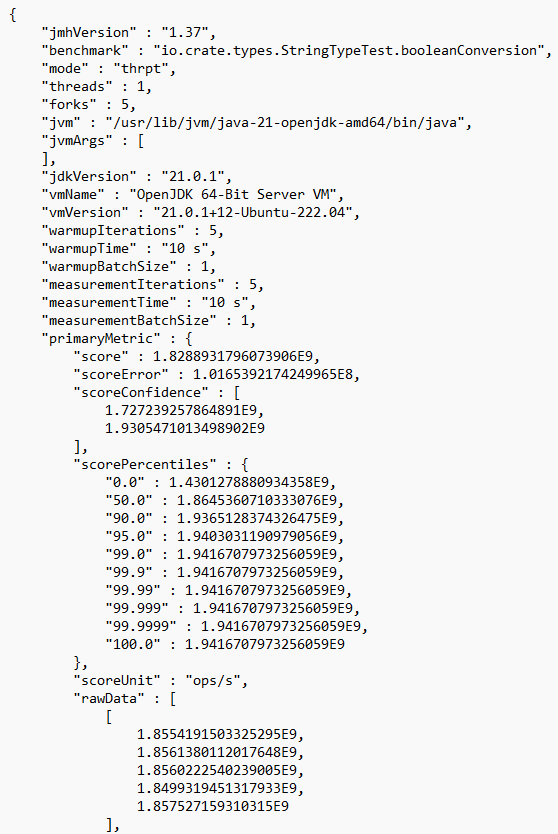
\includegraphics[width=0.6\textwidth]{../img/JMH-example.png}
    \caption{Struktura výsledků měření frameworku JMH}
\end{figure}

Ve výstupním souboru měření pomocí JMH lze nalézt informace o~stroji na~kterém probíhalo měření.
Jedná se především o~název stroje a~verzi operačního systému. Dále zde lze nalézt verzi Javy,
ve~které probíhalo měření. V~souboru je možné vidět také ostatní parametry měření, jako je
zahřívací doba a~počet zahřívacích iterací. Zahřívací iterace jsou zde uvedeny, protože Java
je stejně jako C\# jazyk kompilovaný metodou JIT. Je tedy nutné výstupní data vhodně filtrovat.

Jednotlivé naměřené hodnoty jsou ve výstupním souboru dostupné i~ve~výchozím nastavení JMH.
Naměřené hodnoty nejsou bezrozměrná čísla, ale jsou doplněny i~o~fyzikální jednotku,
kterou naměřená hodnota reprezentuje. Pro~každý běh (fork), přičemž běhů může být v~jednom
spuštění JMH více, se~objeví jedna sada měřených hodnot u~položky \lstinline|rawData|.

\section{Použití statistických metod pro analýzu dat}

Pro vyhodnocování výkonu je využito metod testování hypotéz. Ve statistickém testování
hypotéz se snažíme zamítnout nulovou hypotézu. V~případě zamítnutí nulové hypotézy
se předpokládá, že platí alternativní hypotéza. Popis testování hypotéz v této kapitole
se řídí skripty Pravděpodobnost a~statistika~1 \cite[]{samal_nmai059_nodate}.

Při testování hypotéz rozeznáváme
chyby I. a~II. druhu. Chyba I. druhu znamená, že jsme nulovou hypotézu zamítli,
i~když platí. Chyba II. druhu znamená, že jsme ji nezamítli, ale ona neplatí.

V našem případě porovnávání výkonu bude nulová hypotéza tvrzení, že výkon dvou verzí softwaru je stejný.
Jako alternativní hypotézu budeme uvažovat, že výkony dvou verzí softwaru jsou různé.
Pomocí metody testování hypotéz bude zjišťováno jestli mají dvě spojité náhodné veličiny stejnou střední hodnotu.
Hodnoty spojité náhodné veličiny jsou vždy hodnoty výkonu jedné testované metody programu jedné z verzí.
Pro každou z verzí je tedy uvažovaná jedna náhodná veličina.
Pokud hodnoty těchto veličin mají stejnou střední hodnotu, tak budeme tvrdit, že i výkon obou porovnávaných
verzí je stejný.

Chyba I. druhu tedy v našem případě znamená, že jsme prohlásili, že výkony dvou verzí jsou různé,
ačkoli jsou stejné. Pravděpodobnost chyby I. druhu je obvyklý parametr statistického testu.
Pravděpodobnost chyby I. druhu bude dále značen jako parametr $\alpha$. Parametr $\alpha$
je součástí konfigurace systému PerfEval.

\subsection{Welchův dvouvýběrový t-test}

Welchův dvouvýběrový t-test se používá jako statistika při testování hypotéz.
Tato statistika předpokládá, že náhodné veličiny jsou nezávislé a jejich rozdělení
se blíží normálnímu rozdělení. Nezávislost náhodných veličin je dána vlastnostmi
experimentu \cite[]{twosampletests} a její zajištění je mimo doménu řešeného problému. PerfEval
tedy v~případě použití možnosti t-test možnou závislost zanedbává.

Normalitě náhodných veličin je možné se přiblížit díky centrální limitní větě (CLV).
Se zajištěním normality nám pomůže samotná struktura naměřených výsledků. Výsledky měření
obsahují běhy. Běhy obsahují jednotlivé naměřené hodnoty. Naměřené hodnoty představují
vzorky náhodné veličiny. Pokud se budou v~rámci t-testu namísto naměřených hodnot uvažovat
průměry jednotlivých běhů, tak se podle CLV bude rozdělení těchto průměrů blížit normálnímu rozdělení.


Interval spolehlivosti pro Welchův t-test se spočítá podle následujícího algoritmu. V~algoritmu jsou
použité funkce, které odkazují na skutečně použité knihovní funkce. Funkce mean počítá střední hodnotu
sady hodnot. Funkce var počítá rozptyl sady hodnot. TDistribution je třída, která reprezentuje T-rozdělení
pro statistický test a~parametr konstruktoru je počet stupňů volnosti. Vzorec pro stupně volnosti je dostupný na~Wikipedii
Welchova t-testu \cite[]{enwiki:1184251732}. Vstupními parametry jsou vzorky náhodných veličin a parametr $\alpha$ (critValue.)

\begin{algorithm}[!ht]
    \caption{WelchCI}
    \KwIn{samples1, samples2, critValue}
    \KwOut{lowerBound, upperBound}

    n1 = length(samples1)\;
    n2 = length(samples2)\;

    mean1 = mean(samples1)\;
    mean2 = mean(samples2)\;

    var1 = var(samples1)\;
    var2 = var(samples2)\;

    varOverN1 = var1 / n1\;
    varOverN2 = var2 / n2\;

    degreesOfFreedom = Math.Pow(varOverN1 + varOverN2, 2) / (varOverN1 * varOverN1 / (N1-1) + varOverN2 * varOverN2 / (N2-2))\;

    tDist = new TDistribution(degreesOfFreedom)\;
    tCrit = tDist.inverseCumulativeProbability(critValue / 2)\;
    marginOfError = tCrit * Math.Sqrt(varOverN1 + varOverN2)\;

    lowerBound = mean1 - mean2 - marginOfError\;
    upperBound = mean1 - mean2 + marginOfError\;

\end{algorithm}

Nakonec se již jen zkoumá, zdali tento interval obsahuje nulu.
Pokud interval nulu neobsahuje, pak lze s~pravděpodobností $1-\alpha$ správně tvrdit, že
nulová hypotéza neplatí.

\subsection{Percentilový hierarchický bootstrap}

%% - https://www.youtube.com/watch?v=Xz0x-8-cgaQ

Bootstrap je statistická metoda využívající tzv. resamplování.
Stejně jako u~dvouvýběrového t-testu se předpokládá nezávislost náhodných veličin.
Podmínka nezávislosti bude zanedbána, protože ji není možné zaručit.
Bootstrap se jako metoda používá v~případě, kdy o~náhodných veličinách není možné
určit téměř žádné silné předpoklady. Díky této vlastnosti je bootstrap pro testování
hypotéz o~výkonu verzí softwaru použit.

\begin{algorithm}[!ht]
    \caption{Bootstrap1D}
    \KwIn{measurements, iterationCount}
    \KwOut{bootstrappedSamples}
    
    n = length(measurements)\;
    samples = []\;

    \For{i = 0; i < iterationCount; i += 1}{
        sum = 0\;
        \For{j = 0; j < n; j = j + 1}{
            index = random() mod n\;
            sum += measurements[index]\;
        }
        samples.add(sum/n)\;
    }
    
    \Return{samples}\;
\end{algorithm}

\begin{algorithm}[!ht]
    \caption{Bootstrap2D}
    \KwIn{runs1, runs2, iterationCount}
    \KwOut{bootstrappedSamples}
    
    n = length(runs1)\;
    m = length(runs2)\;
    samples = []\;
    
    \For{i = 0; i < iterationCount; i += 1}{
        samples1 = []\;
        \For{j = 0; j < n; j += 1}{
            index = random() mod n\;
            samples1.add(Bootstrap1D(runs1[index], 1))\;
            }
        samples2 = []\;
        \For{k = 0; k < m; k += 1}{
            index = random() mod m\;
            samples2.add(Bootstrap1D(runs2[index], 1))\;
        }
        diff = mean(samples1)-mean(samples2)\;
        samples.add(diff)\;
    }
    
    \Return{samples}\;
\end{algorithm}

Podle percentilového bootstrapu se interval spolehlivosti nalezne tak, že se hranice intervalu stanoví jako $\frac{\alpha}{2}$-tý
a~$\frac{1-\alpha}{2}$-tý percentil z~resamplovaného souboru. Tyto dvě hodnoty budou představovat hranice intervalu.

Zkoumanou náhodnou veličinou je rozdíl dvou náhodných veličin. Tyto dvě náhodné veličiny jsou dány měřením
výkonnosti dvou verzí softwaru. Nulová hypotéza, která je vyvracena, tvrdí, že obě veličiny mají stejnou střední hodnotu.
Pokud tedy interval spolehlivosti neobsahuje nulu, tak můžeme nulovou hypotézu vyvrátit, protože s~pravděpodobností
$1-\alpha$ o ní test správně prohlásil, že neplatí.

Naměřené vzorky však nejsou prostý statistický soubor. Jedná se o~hierarchický soubor dat.
Každé jedno měření se skládá z~jednoho, nebo více běhů. Každý běh se skládá z~jednoho, nebo více naměřených údajů.
Vytváření bootstrapového statistického souboru tedy vypadá trochu odlišně.

Bootstrap2D ukazuje, jak vypadá výběr nového statistického souboru. Vyberou
se náhodné běhy z~jednotlivých výsledků měření. Z těchto běhů se získá 1D bootstrap.
Novým prvkem vytvářeného statistického souboru se stane rozdíl těchto bootstrapů.

\subsection{Co dělat v případě nevyvrácení hypotézy?}

V~případě nevyvrácení nulové hypotézy nám statistické testy nedávají žádnou informaci.
Nicméně je stále nutné se rozhodnout, zdali nulová hypotéza platí. Je nutné se ale stále
vyvarovat chyby II. druhu. Proto v tomto případě budeme považovat nulovou hypotézu za platnou,
pokud bude interval spolehlivosti dostatečně úzký. Pokud má tedy interval spolehlivosti
dolní mez $D_{LOW}$ a horní mez $D_{HIGH}$, pak je jeho šířka $D_{HIGH}-D_{LOW}$. Odhadovaný průměr by byl $\frac{D_{HIGH}+D_{LOW}}{2}$.
Relativní šířka intervalu je tedy poměr šířky a průměru, tedy $\frac{2\cdot(D_{HIGH}-D_{LOW})}{D_{HIGH}+D_{LOW}}$.

V případě většího množství vzorků je možné zužovat interval spolehlivosti. Vztah mezi
šířkou a~počtem vzorků odpovídá $O(\frac{1}{\sqrt{n}})$, kde $n$ je počet vzorků. Z~daného
množství vzorků je tedy možné odhadnout, kolik vzorků je ještě zapotřebí změřit.

V případě, že je interval dostatečně úzký, prohlásíme, že nulová hypotéza platí.
V případě, že interval není dostatečně úzký, prohlásíme, že vzorků není dost.

PerfEval tedy v~konečném důsledku rozlišuje tři základní výsledky porovnání výkonu verzí.
Test končí s~kladným výsledkem, pokud platí nulová hypotéze dle kritérií výše. Test
končí s~kladným výsledkem také když je nulová hypotéza vyvrácena, ale výkon novější verze je lepší.
V~ostatních případech test neprojde. Další dva možné výsledky testu tedy budou značit selhání.
Druhý výsledek testu značí, že~nulová hypotéza neplatí, a~zároveň, že~došlo ke~zhoršení výkonu.
Třetí výsledek značí, že~se~nulovou hypotézu nepodařilo vyvrátit, ale~počet naměřených výsledků
je~příliš malý.
